\section{Task 1}

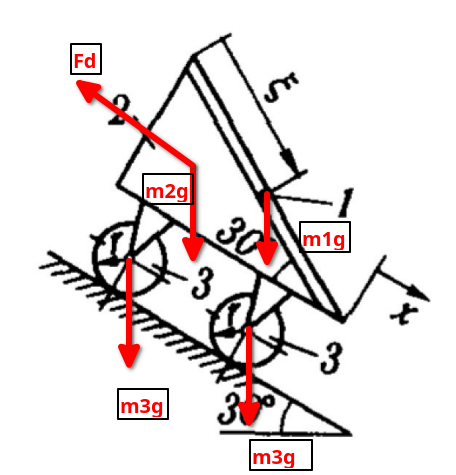
\includegraphics[width=\linewidth]{task1.png}

\subsection{Derivation of points positions}

\begin{enumerate}
    \item I assume that point $O_1$ is positioned in the (0, 0).
    \item We can describe the position of point $A$ as it rotates around point $O_1$ as follows:
          \begin{align}
              \vec{r_A(t)} = O_1A \begin{bmatrix}
                  \cos(\phi) \\
                  \sin(\phi)
              \end{bmatrix}
          \end{align}
    \item Position of $O_2$ is $(-c, a)$ as follows from task description.
    \item We can describe the position of point $B$ as intersection between two circles: first with center at $A$ and radius $AB$ and second with center at $O_2$ and radius $OA_2$:
          \begin{align}
              \begin{cases}
                  (x_B - x_A)^2 + (y_B - y_A)^2 = AB^2 \\
                  (x_B - x_{O_2})^2 + (y_B - y_{O_2})^2 = O_2A^2
              \end{cases}
          \end{align}
          These equations can be solved easily with solvers like $Sympy$ for $Python$.
          I faced several problems with this step:
          \begin{enumerate}
              \item Mechanism does not work for all angles of $\phi$.
                    Distance between $A$ and $O_2$ is at maximum:
                    \begin{align}
                        (O_1A \cdot \cos(\phi) - a)^2 + (O_1A \cdot \sin(\phi) + c)^2 = (AB + O_2B)^2
                    \end{align}
                    This will happen when $O_2BA$ will form a straight line.
                    \href{https://www.wolframalpha.com/input?i=%2821+*+cos%28x%29+-+56%29%5E2+%2B+%2821+*+sin%28x%29+%2B+26%29%5E2+%3D+%2854+%2B+25%29%5E2}{Wolframagic solution link}
                    We get 2 angles, but actually only one is important for us, because we rotate CCW starting from $\pi/3$.
                    Limit angle will be $\approx 2.004$ radians. Thus my simulation is limited for $\phi \in [\pi/3, 2.004]$.
              \item We have 2 solutions from quadratic equations and have to choose one:
                    I select the most right and top (greatest $x$ and $y$ coordinates) point because it looks nicer and closer to starting position from picture.
                    I will follow this approach for other cases too.
          \end{enumerate}

    \item We can describe the position of point $C$ as intersection between two circles: first with center at $B$ and radius $BC$ and second with center at $A$ and radius $AB$:
          \begin{align}
              \begin{cases}
                  (x_C - x_B)^2 + (y_C - y_B)^2 = BC^2 \\
                  (x_C - x_A)^2 + (y_C - y_A)^2 = AB^2
              \end{cases}
          \end{align}

    \item We can describe the position of point $D$ as intersection between circle (center $C$ radius $CD$) and a line because point D has only translational motion on the fixed axis:
          \begin{align}
              \begin{cases}
                  (x_D - x_C)^2 + (y_D - y_C)^2 = CD^2 \\
                  y_D = d
              \end{cases}
          \end{align}

    \item Point $E$ is on $CD$ segment and can be found as follows:
          \begin{align}
              \vec{r_E(t)} = \vec{r_C(t)} + \frac{\vec{r_D(t)} - \vec{r_C(t)}}{CD} CE
          \end{align}

    \item Point $F$ can be found as intersection of two circles: one with center $E$ and radius $EF$ and second with center $O_3$ and radius $O_3F$:
          \begin{align}
              \begin{cases}
                  (x_F - x_E)^2 + (y_F - y_E)^2 = EF^2 \\
                  (x_F - x_{O_3})^2 + (y_F - y_{O_3})^2 = O_3F^2
              \end{cases}
          \end{align}


\end{enumerate}

\subsection{Derivation of velocities for points}
\href{https://www.youtube.com/watch?v=l7jCZV_lIHM}{meme link}

\begin{enumerate}
    \item Velocity of point $A$
          Obviously, it is a rotation around point $O_1$:
          \begin{align}
              \vec{v_A(t)} = \omega \cdot O_1A \cdot \begin{bmatrix}
                  -\sin(\phi) \\
                  \cos(\phi)
              \end{bmatrix}
          \end{align}

    \item Velocity of point $B$ can be found as follows:
          \begin{align}
              \vec{v_B}(t) = \dot{\vec{r_B}}(t)
          \end{align}
    \item Velocity of point $C$ can be found as follows:
          \begin{align}
              \vec{v_C}(t) = \dot{\vec{r_C}}(t)
          \end{align}

    \item Velocity of point $D$ can be found as follows:
          \begin{align}
              \vec{v_D}(t) = \dot{\vec{r_D}}(t)
          \end{align}

    \item Velocity of point $E$ can be found as follows:
          \begin{align}
              \vec{v_E}(t) = \dot{\vec{r_E}}(t)
          \end{align}

    \item Velocity of point $F$ can be found as follows:
          \begin{align}
              \vec{v_F}(t) = \dot{\vec{r_F}}(t)
          \end{align}



\end{enumerate}

\subsection{Derivation of angular velocities}

Let's start with meme:


\includegraphics[width=120px]{meme.jpg}

\begin{enumerate}
    \item We could use IC(instanteneous centre of zero velocity to simplify our calculations,
          but I will not do it because we already have all velocities and positions of points and it is enough.
    \item For angular velocities we can use this formula:
          \begin{align}
              \vec{v_1}(t) = \vec{v_2}(t) + \vec{\omega}(t) \times \vec{r_{12}}(t)
          \end{align}
    \item Angular velocity of $O_1A$:
          \begin{enumerate}
              \item $O_1A$ is a fixed point and we know from description that $\omega = 2$.
              \item But nevertheless:
                    \begin{align}
                        \vec{v_A}(t) = \vec{v_{O_1}}(t) + \vec{\omega_{O_1A}}(t) \times \vec{r_{O_1A}}(t) \\
                        \omega_{O_1A} = \frac{|\vec{v_A}(t) - \vec{v_{O_1}}(t)|}{|\vec{r_{O_1A}}(t)|}
                    \end{align}
              \item In simulation I compute both variants, and they almost equal
                    with respect to precision of simulation and derivative computation algorithm (I use the easiest).
          \end{enumerate}
    \item As all formulas are pretty much the same I will not comment others.
    \item Angular velocity of $O_2B$:
          \begin{align}
              \vec{v_B}(t) = \vec{v_{O_2}}(t) + \vec{\omega_{O_2B}}(t) \times \vec{r_{O_2B}}(t) \\
              \omega_{O_2B} = \frac{|\vec{v_B}(t) - \vec{v_{O_2}}(t)|}{|\vec{r_{O_2B}}(t)|}
          \end{align}
    \item Angular velocity of $AB$:
          \begin{align}
              \vec{v_B}(t) = \vec{v_A}(t) + \vec{\omega_{AB}}(t) \times \vec{r_{AB}}(t) \\
              \omega_{AB} = \frac{|\vec{v_B}(t) - \vec{v_A}(t)|}{|\vec{r_{AB}}(t)|}
          \end{align}
    \item Angular velocity of $BC$ and $AC$:
          As $ABC$ form a fixed triangle, their angular velocities are equal:
          \begin{align}
              \omega_{AB} = \omega_{BC} = \omega_{AC}
          \end{align}
          But in order to justify and prove it to myself I also compute them separately:
          \begin{align}
              \vec{v_C}(t) = \vec{v_B}(t) + \vec{\omega_{BC}}(t) \times \vec{r_{BC}}(t) \\
              \omega_{BC} = \frac{|\vec{v_C}(t) - \vec{v_B}(t)|}{|\vec{r_{BC}}(t)|}
          \end{align}
          \begin{align}
              \vec{v_C}(t) = \vec{v_A}(t) + \vec{\omega_{AC}}(t) \times \vec{r_{AC}}(t) \\
              \omega_{AC} = \frac{|\vec{v_C}(t) - \vec{v_A}(t)|}{|\vec{r_{AC}}(t)|}
          \end{align}
    \item Angular velocity of $CD$:
          \begin{align}
              \vec{v_D}(t) = \vec{v_C}(t) + \vec{\omega_{CD}}(t) \times \vec{r_{CD}}(t) \\
              \omega_{CD} = \frac{|\vec{v_D}(t) - \vec{v_C}(t)|}{|\vec{r_{CD}}(t)|}
          \end{align}
    \item Angular velocities of $CE$ and $ED$:
          $CDE$ are on the same "body" and their angular velocities are equal:
          \begin{align}
              \omega_{CD} = \omega_{CE} = \omega_{ED}
          \end{align}
    \item Angular velocity of $EF$:
          \begin{align}
              \vec{v_F}(t) = \vec{v_E}(t) + \vec{\omega_{EF}}(t) \times \vec{r_{EF}}(t) \\
              \omega_{EF} = \frac{|\vec{v_F}(t) - \vec{v_E}(t)|}{|\vec{r_{EF}}(t)|}
          \end{align}
    \item Angular velocitiy of $O_3F$:
          \begin{align}
              \vec{v_F}(t) = \vec{v_{O_3}}(t) + \vec{\omega_{O_3F}}(t) \times \vec{r_{O_3F}}(t) \\
              \omega_{O_3F} = \frac{|\vec{v_F}(t) - \vec{v_{O_3}}(t)|}{|\vec{r_{O_3F}}(t)|}
          \end{align}
\end{enumerate}

\subsection{Accelerations for $A$ and $B$}

\begin{enumerate}
    \item Acceleration of $A$:
          \begin{align}
              \vec{a_A}(t) = \dot{\vec{v_A}}(t)
          \end{align}
          We can mention that as $\omega$ is const, there will be no tangential acceleration for $A$.
          In simulation we can see very small tangential acceleration, but it is because of precision of simulation.
    \item Tangential acceleration of $A$:
          \begin{align}
              \vec{a_{At}}(t) = \frac{\vec{a_A}(t) \cdot \vec{v_{A}}(t)}{|\vec{v_{A}}(t)|} \vec{r_{A}}(t)
          \end{align}
    \item Normal acceleration of $A$:
          \begin{align}
              \vec{a_{An}}(t) = \vec{a_A}(t) - \vec{a_{At}}(t)
          \end{align}
    \item Acceleration of $B$:
          \begin{align}
              \vec{a_B}(t) = \dot{\vec{v_B}}(t)
          \end{align}
    \item Tangential acceleration of $B$:
          \begin{align}
              \vec{a_{Bt}}(t) = \frac{\vec{a_B}(t) \cdot \vec{v_{B}}(t)}{|\vec{v_{B}}(t)|} \vec{r_{B}}(t)
          \end{align}
    \item Normal acceleration of $B$:
          \begin{align}
              \vec{a_{Bn}}(t) = \vec{a_B}(t) - \vec{a_{Bt}}(t)
          \end{align}
\end{enumerate}